\documentclass[11pt, a4paper]{scrartcl}
\usepackage[ngerman]{babel}
%\usepackage[T1]{fontenc}
\usepackage[utf8]{inputenc}
\usepackage{lmodern}
\usepackage{amsmath}
\usepackage{amssymb}
\usepackage{amsthm}
\usepackage{graphicx}
\usepackage{listings}
\usepackage{booktabs}
\usepackage{float}
\usepackage{pdfpages}
\usepackage{cite}
\usepackage{url}
\bibliographystyle{unsrtnat}
\usepackage[numbers]{natbib}
\usepackage[T1]{fontenc}
%
\begin{document}
\lstset{basicstyle=\small,
		 inputencoding=latin1,
		stringstyle=\ttfamily,
		identifierstyle=,
		showstringspaces=false,
		language=c,
		frame=trBL}
%
\subsection*{TI III WS 2013, Fr. 12-14}
\section*{Lösung Übungsblatt 7}
\textbf{Christoph van Heteren-Frese (Matr.-Nr.: 4465677), Julien  Stengel } \\%(Matr.-Nr.: 4567553)}\\
Tutor: Ruhland, eingereicht am \today\\
\hrule
%
\section*{Aufgabe 1}
\begin{figure}[H]
\center
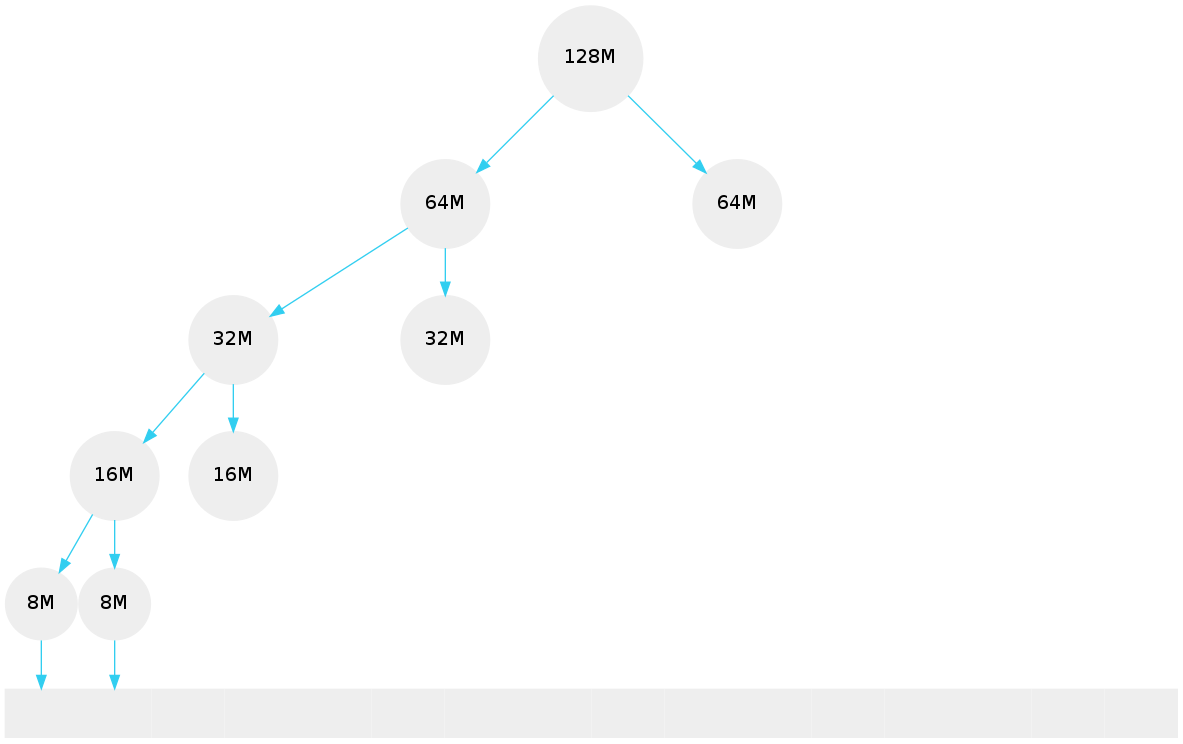
\includegraphics[scale=0.32]{a1_1}
\caption{Anforderung A: 6MB}
\end{figure}
\begin{figure}[H]
\center
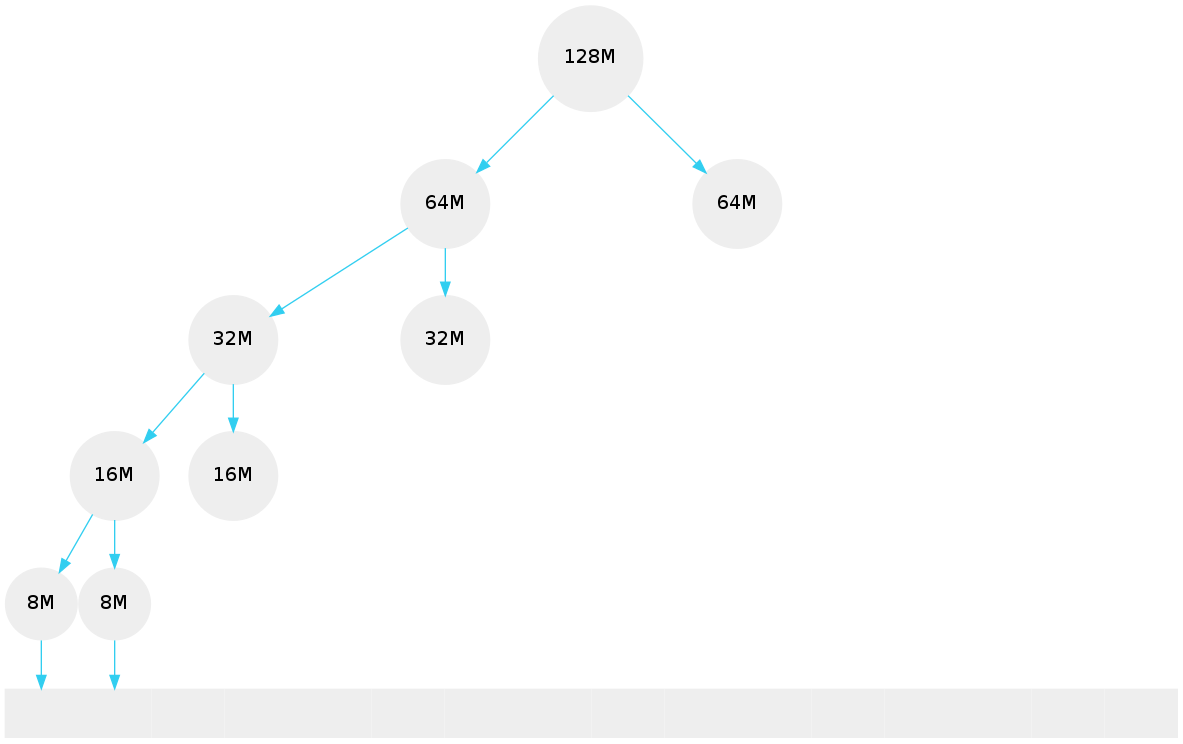
\includegraphics[scale=0.32	]{a1_1}
\caption{Anforderung B: 4MB}
\end{figure}
\begin{figure}[H]
\center
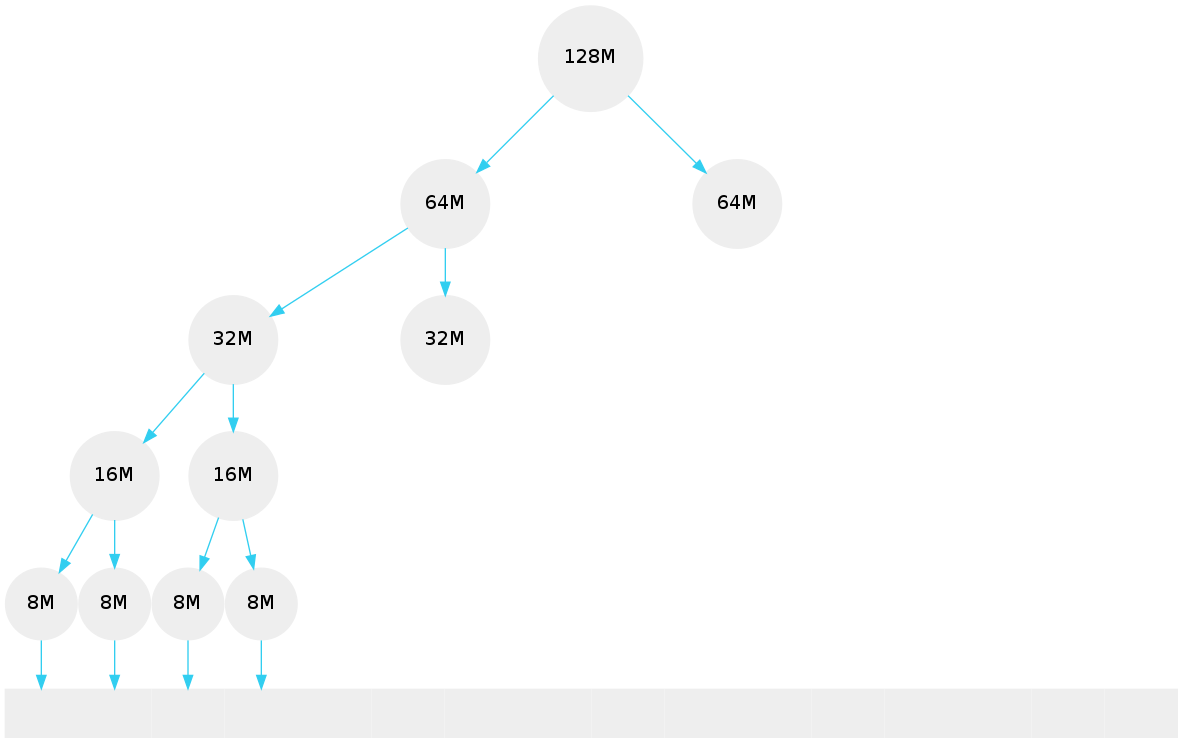
\includegraphics[scale=0.32]{a1_2}
\caption{Anforderung C: 8MB}
\end{figure}
\begin{figure}[H]
\center
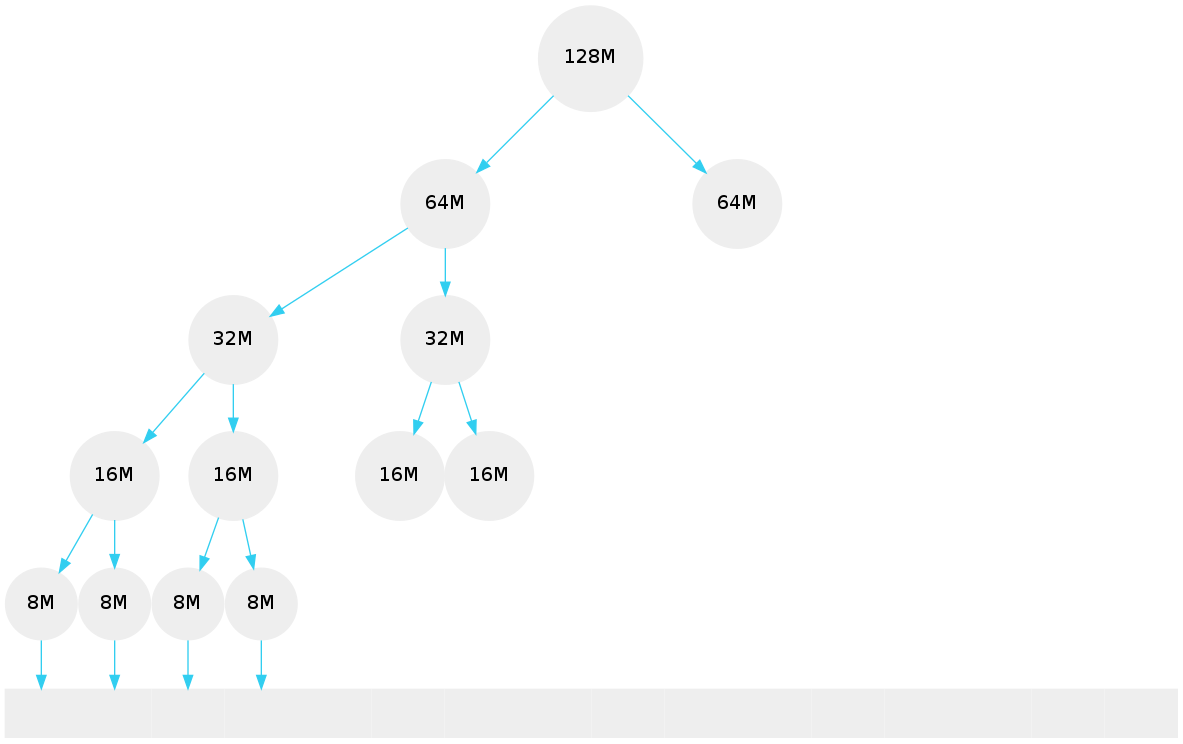
\includegraphics[scale=0.32]{a1_3}
\caption{Anforderung D: 16MB}
\end{figure}
\begin{figure}[H]
\center
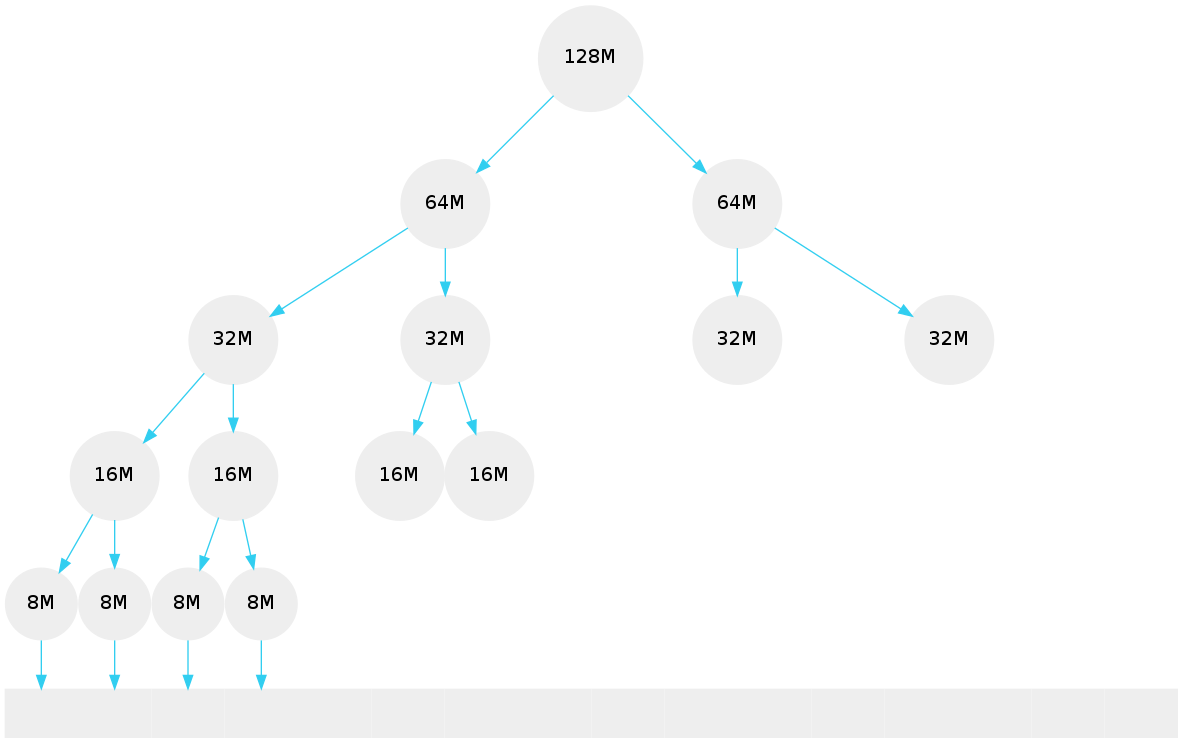
\includegraphics[scale=0.32]{a1_4}
\caption{Anforderung E: 32MB}
\end{figure}
\begin{figure}[H]
\center
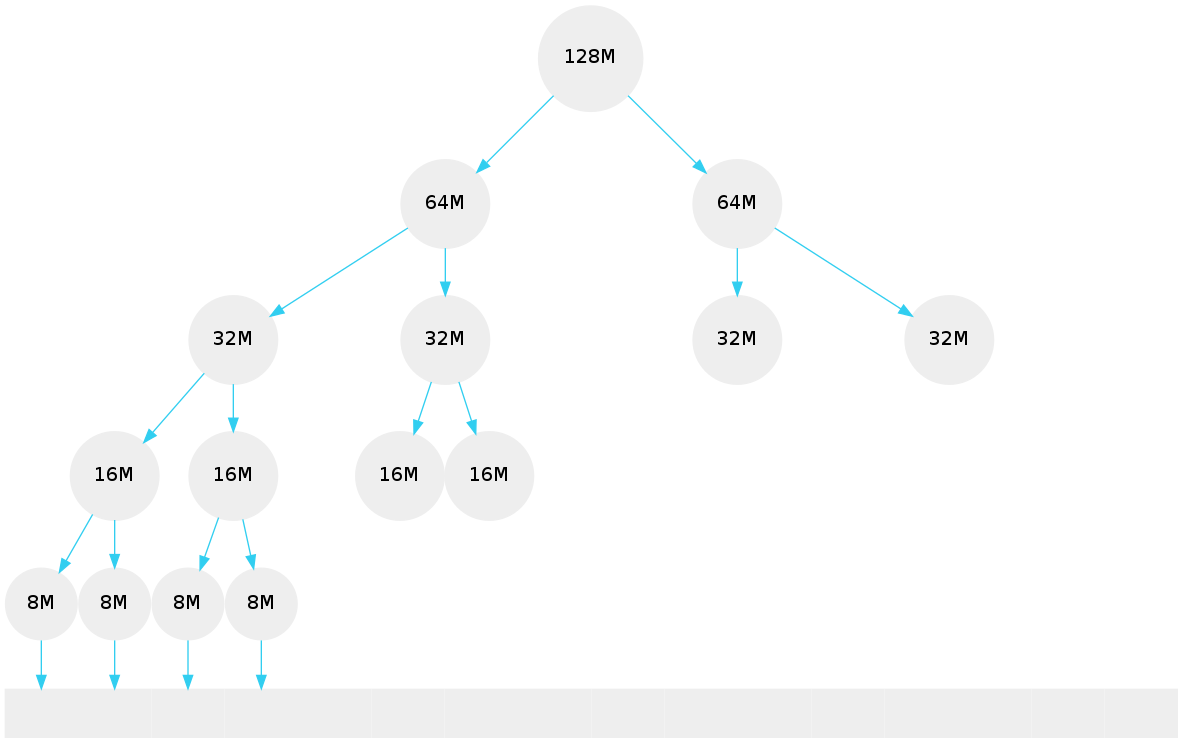
\includegraphics[scale=0.32]{a1_4}
\caption{Freigabe A}
\end{figure}
\begin{figure}[H]
\center
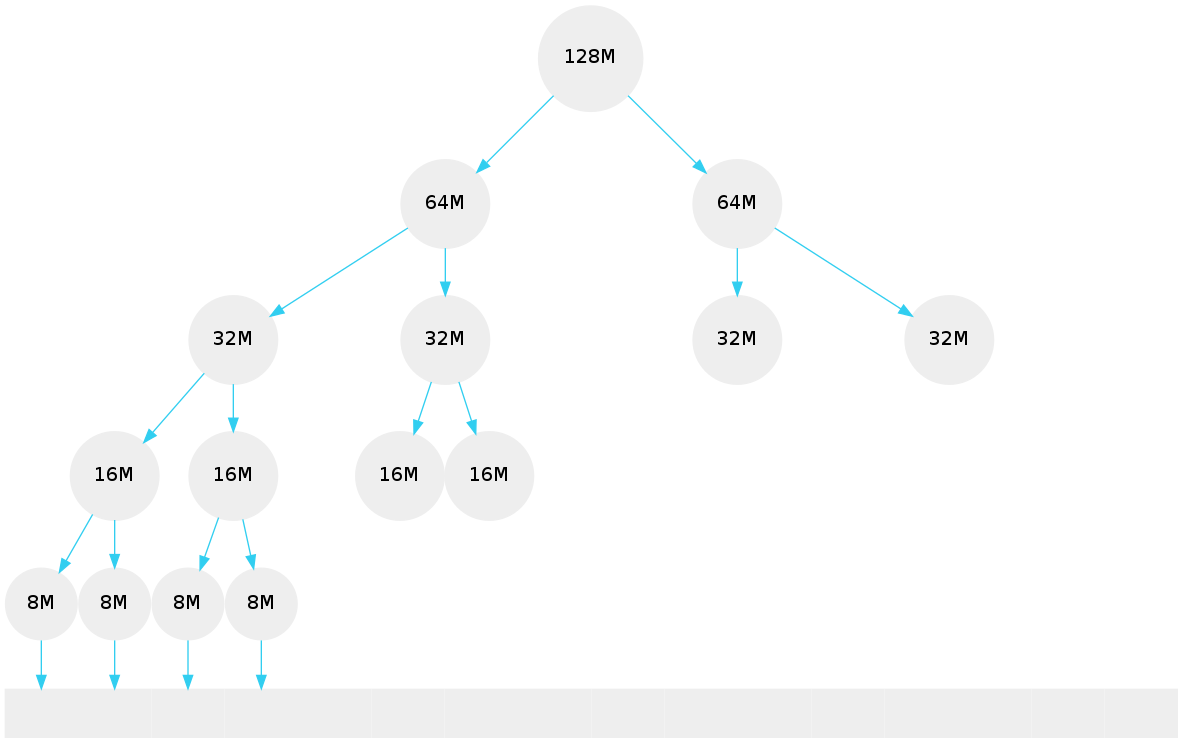
\includegraphics[scale=0.32]{a1_4}
\caption{Anforderung F: 16MB}
\end{figure}
\begin{figure}[H]
\center
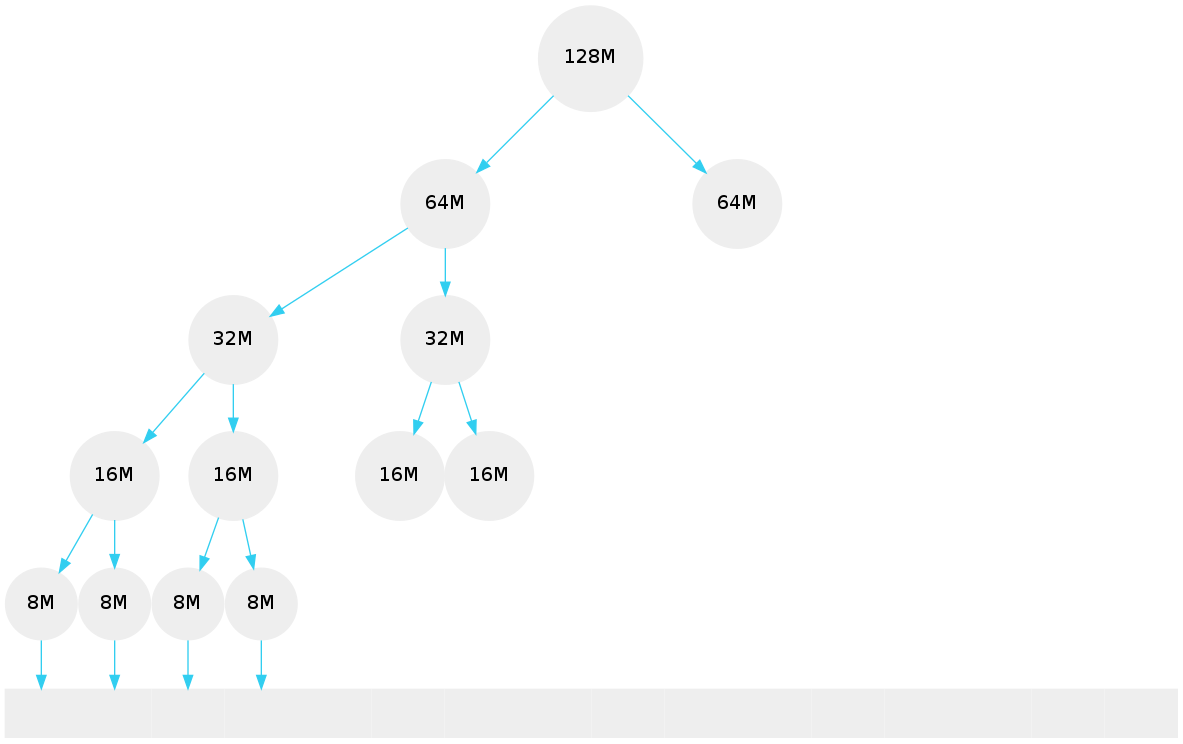
\includegraphics[scale=0.32]{a1_5}
\caption{Freigabe von E}
\end{figure}
\begin{figure}[H]
\center
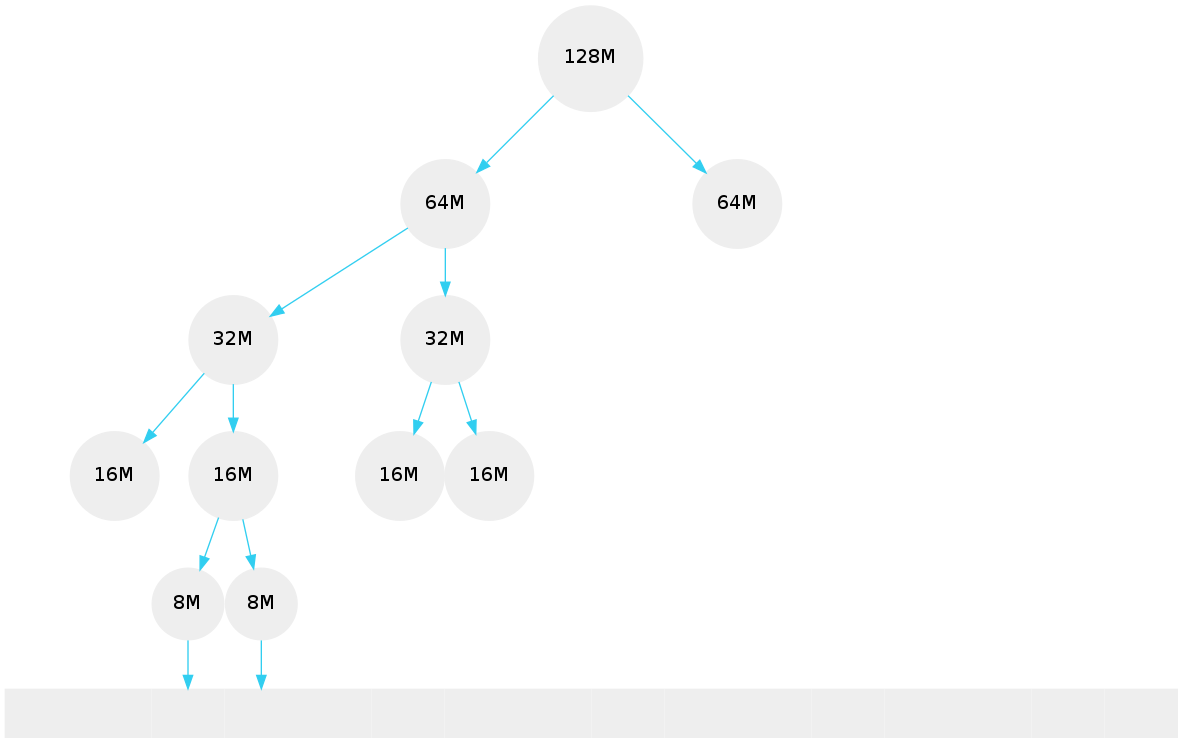
\includegraphics[scale=0.32]{a1_6}
\caption{Freigabe von B}
\end{figure} 	
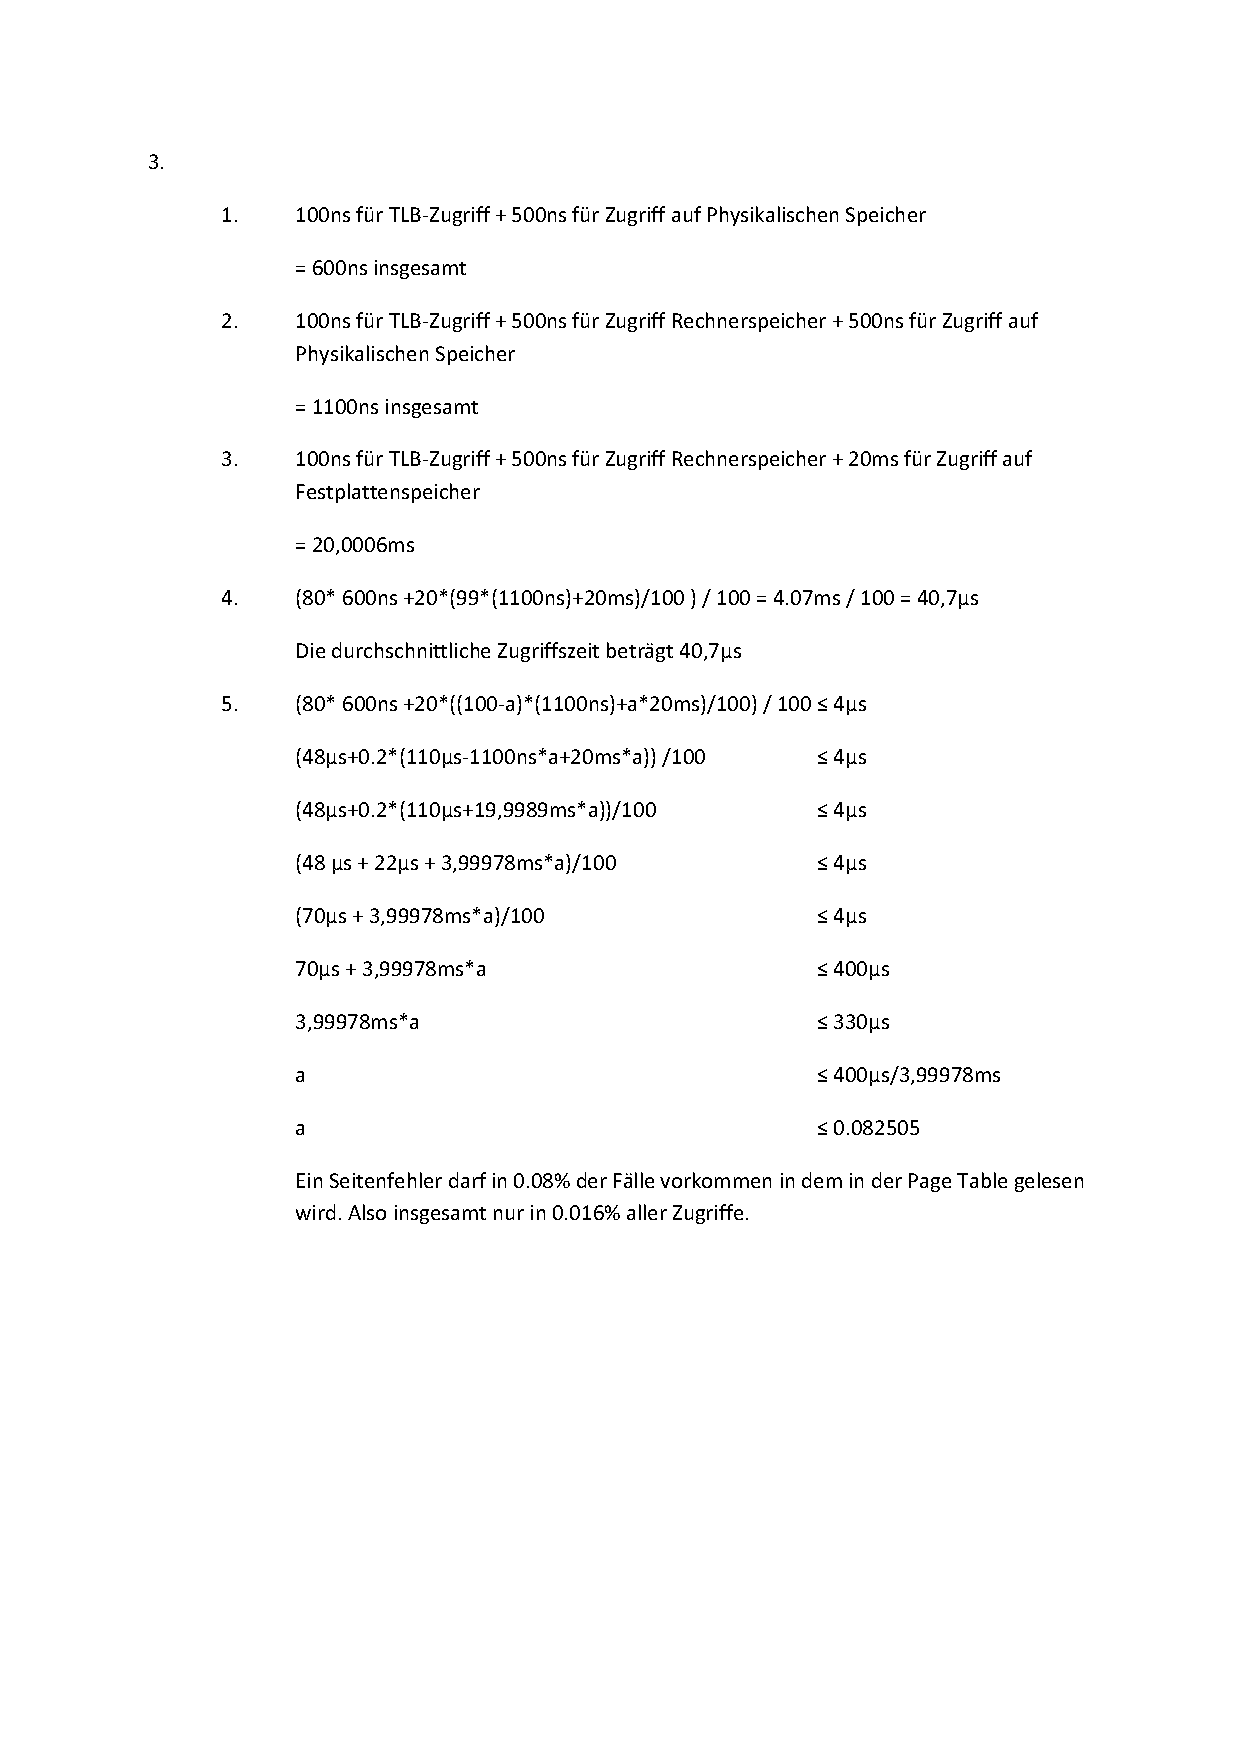
\includepdf[pages={1}]{../uebung7.pdf}
\bibliography{ti3}
\end{document}
